\section{Introduction}
\label{sec:introduction}
%NOTE: General Background of MEC and Motivation
Edge computing is a promising solution for increasing computation-intensive and energy-hungry applications on mobile devices.
Large amount of mobile devices can connect to the access points (APs) which function as gateways to aggregate and dispatch jobs to the edge servers \cite{MEC-SURVEY}.
The edge servers are deployed in closer proximity to APs than cloud infrastructure, which alleviate the communication overhead and enable the computation of time-sensitive jobs.
However, the edge servers are usually deployed with limited computation resources.
The establishment of efficient cooperation among edge servers is one of the major design challenges, given the signaling overhead and latency of distributed information exchange and decision making.
%given the network transmission latency and signaling overhead

\begin{figure}[htp!]
    \centering
    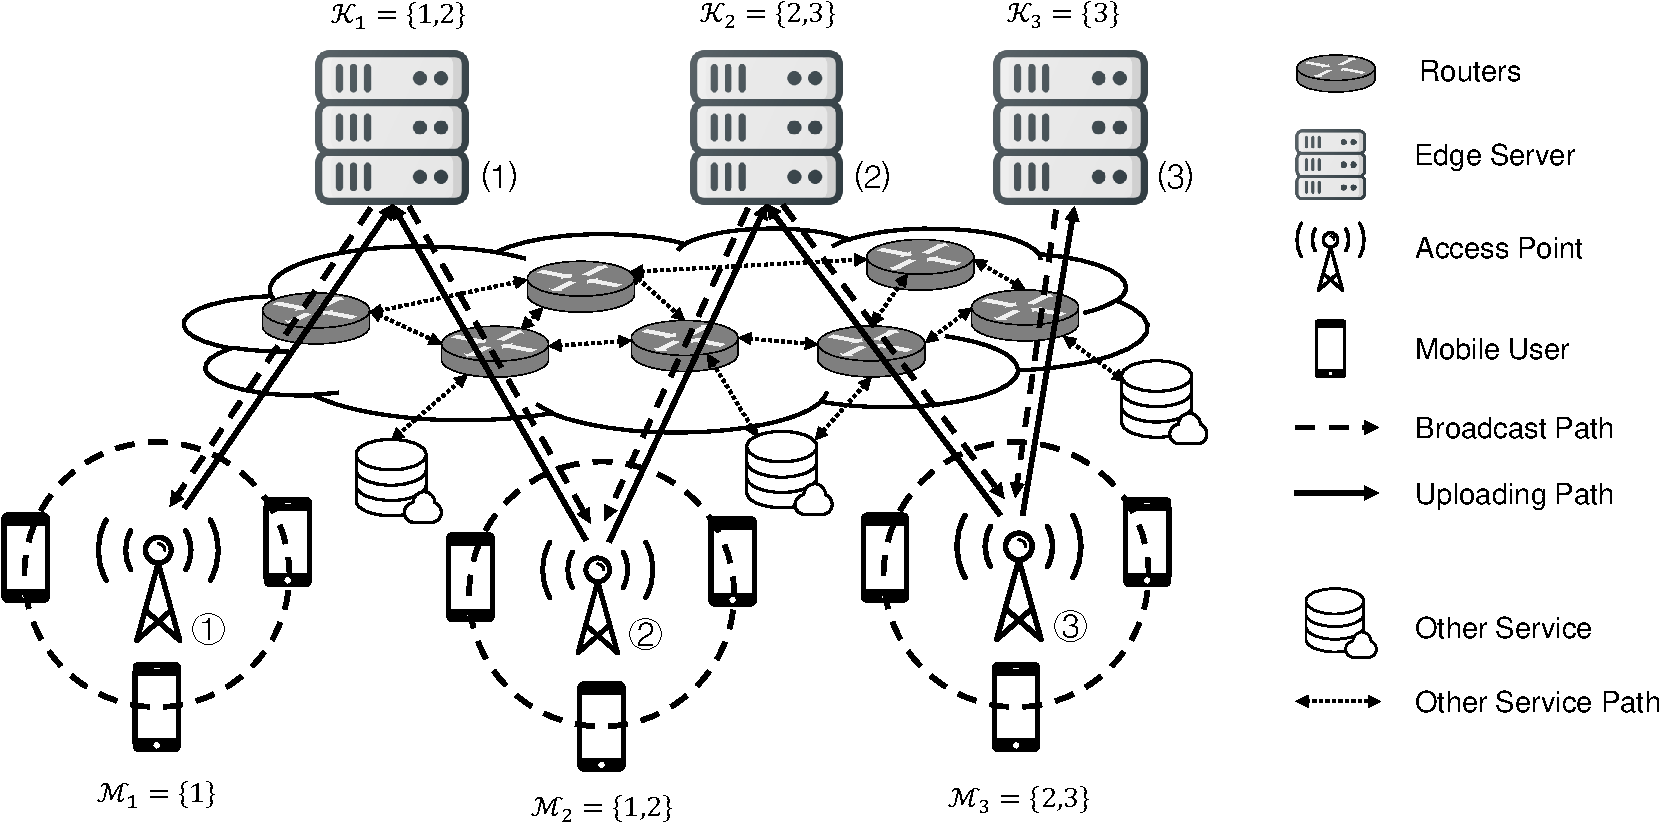
\includegraphics[width=0.45\textwidth]{system-model.pdf}
    \caption{The Illustration of System Model}
    \label{fig:system}
\end{figure}

%NOTE: Motivation with MAN
We consider an edge computing system with multiple APs and edge servers residing in the Metropolitan Area Network (MAN).
The APs collect jobs offloaded from the mobile users in its service area and make dispatching decision for each job. According to the MAN performance analysis in \cite{MAN-LATENCY}, the data transmission latency {among APs and edge servers} varies a lot with respect to different hours of day and devices' locations in a MAN. {In addition, each AP also suffers from signaling latency, which is the time consumed for each AP to collect system state information under some signaling mechanism.}
There has been a number of existing literature considering random transmission latency of job delivery in edge computing networks (e.g., \cite{latency-EDGE19,MOBIHOC19-ZhouZ,IOTJ18-FanQ,TOC19-LiuC,JSAC19-AlameddineHA}). 
\tann{However, there are only a few works considering signaling latency of cooperation among distributed job dispatchers \cite{JSAC17-LyuX,TWC18-LyuX}.}
In fact, it is full of challenge to consider latency in {both job delivery and} signaling. The cooperation of distributed dispatchers suffers from significant unpredictable signaling and transmission overhead. Therefore, aggregating the global system state information at each AP is not practical, and a centralized dispatcher design is discouraged. Moreover, the latency will also lead to outdated information at each dispatcher and information inconsistency among different dispatchers\comments{, which may introduce ineliminable estimation error on the number of jobs in the system and thus discourage the cooperative dispatcher design}.
%\setlength{\leftmargini}{0pt}
% \begin{enumerate}[leftmargin=*]
%     \item Firstly, the centralized dispatcher design is discouraged for outdated system information and unpredictable \tann{signaling latency}.
%     \item Secondly, the cooperation of distributed dispatchers suffers from significant signaling overhead. Therefore, aggregating the global system state information at each AP is not practical.
%     \item  Finally, the transmission latency causes the inconsistency of system information at different dispatchers.
% \end{enumerate}

%NOTE: Our contributions
In this paper, we would like to shed some lights on the above challenging distributed dispatcher design via proposing the POMDP (partially observable Markov decision process) problem formulation and a novel low-complexity approximate MDP solution framework.
Specifically, we consider a practical scenario where the signaling latency among APs and edge servers as well as job uploading latency from APs to edge servers are assumed to be random, and each AP can only receive the broadcast state information from part of the APs with random latency (i.e., the global system state is not available at the APs).
Our main contributions in this new optimization scenario are summarized as follows.
\begin{itemize}
    \item %NOTE: novel solution framework
    We propose a novel low-complexity distributed solution framework for the dispatcher design at APs.
    By leveraging partial observation at each dispatcher, we derive the expression of approximate value function under MDP framework and decouple the optimization problem onto each AP.
    % we directly derive the expression of approximate value function and the distributed dispatching policies at all the edge servers which can be facilitated via partial and local knowledge of the approximate value function.
    Thus, the complicated POMDP solution is avoided.
    To our best knowledge, this is the first work to address the cooperative distributed multi-agent optimization problem with outdated and partial information under MDP framework.
    \item %NOTE: performance guarantee
    We derive an analytical cost lower bound for the proposed distributed dispatching policy in the above low-complexity solution framework.
    In the conventional approximate MDP methods, the solution is usually evaluated via numerical method which are hard to obtain analytical performance bound.
    \item We conduct extensive simulations based on the Google Cluster trace, compared with three heuristic benchmarks. The evaluation results show that our proposed job dispatching policy can achieve $20.67\%$ reduction in average job response time, and our algorithm consistently performs well under various parameter settings of signaling latency, job arrival intensity and job processing time.
\end{itemize}

\noindent \textbf{Paper Organization: }The remainder of this paper is organized as follows.
In Section \ref{sec:review}, the related works are elaborated.
In Section \ref{sec:model}, we illustrate the system model and the signaling model with random latency.
In Section \ref{sec:formulation}, we formulate the global optimization of dispatching decisions at all APs as an POMDP.
In Section \ref{sec:algorithm}, we introduce the novel low-complexity distributed solution framework for the above POMDP.
The numerical analysis of the proposed solution is provided in Section \ref{sec:evaluation}, and the conclusion is drawn in Section \ref{sec:conclusion}.

\section{Related Work}
\label{sec:review}
%NOTE: resource placement (cache-like problem), service migration
% {
%     There have been a number of works focusing on the resource allocation, job dispatching and service migration of edge computing system.
%     For example, in \cite{TON19-WangSq}, the edge servers are one-to-one bound to the base stations (BSs), and the job migration could be applied according to users' mobility traces via the backhaul network connecting the BSs.
%     However, according to a recent research \cite{INFOCOM19-WuC}, the resource re-allocation for running jobs on servers is hard to implement in practice, as it is hard for jobs migration among heterogeneous edge servers with different resource configurations.
%     Hence, it might be more important to optimize the job dispatching strategy at their arrival time.
% }

%NOTE: single-agent dispatching, single UE/server
There have been a number of works considering the centralized job dispatching with updated and complete knowledge on the states of edge computing systems.
For example, in order to minimize the average job response time in the worst case, the authors in \cite{tan-online} designed an online algorithm for job dispatching in edge computing systems with fixed uploading latency.
In the scenario that APs and edge servers are connected via software defined network (SDN), the authors in \cite{IOTJ18-FanQ} proposed a heuristic algorithm to dispatch the jobs to the closest edge servers according to their locations.
Considering random jobs arrival and job offloading to a single edge server, the authors in \cite{mdp-globecom,mdp-tvt} formulate the offloading problem as an infinite-horizon Markov decision process (MDP).
% When the jobs can be dispatched to either edge servers or cloud servers with fixed uploading latency, the authors in \cite{MASS18-MengZ} formulated job dispatching problem as an integer linear programming to minimize the total uploading latency.
In the above works, a centralized dispatcher with complete and updated knowledge of the system status was assumed in the edge computing systems, which might be impractical.

Hence, there are also some works considering the distributed job dispatching in edge computing systems.
For example, in order to minimize a weighted sum of total energy consumption and uploading latency, the authors in \cite{ToN-Xuchen2016} proposed a distributed job dispatching algorithm based on game theory to achieve the Nash equilibrium. 
Considering job migration at edge servers, the authors in \cite{ToN-xujie2018} optimized the edge computing performance in a distributed manner with limited energy resources via a congestion game framework.
In the scenario that APs cooperatively dispatch jobs with multiple edge servers, the authors in \cite{mdp-jcin} proposed a novel approximate MDP solution framework to alleviate the algorithm complexity and minimize the average job response time.
However, in the above works, the latency of information exchange among APs and edge servers is ignored.
In fact, due to the complicated network traffic, this latency might be significant, and the staleness of system state information at the dispatcher of a edge computing systems should be considered.

%NOTE: stale-information based multi-agent related works
The staleness of information sharing among APs and edge servers may degrade the performance of the job dispatching algorithm in edge computing systems.
To the best of our knowledge, there are very limited works investigating this issue.
For example, the authors in \cite{JSAC17-LyuX} proposed a randomized policy via Lyapunov optimization approach to stabilize the queues in a MEC system with multiple IoT devices offloading jobs to one edge server, where \brlatency~is considered. 
In \cite{TWC18-LyuX}, the above approach was applied to the scenario that mobile devices offload jobs to each other via D2D link.
In the above two works, there is one centralized dispatcher in the system and the objective is to stabilize the transmission queues.
Hence, the existence of \brlatency~may not raise significant challenge to the algorithm designs.

However, the design of distributed dispatchers with \brlatency~could be more challenging.
For example, the signaling latency at distributed dispatchers could be different, and the synchronization of their dispatching decisions become infeasible.
Furthermore, taking the signaling overhead in consideration, it is of more practical significance favor for the distributed dispatchers to make decisions based on locally observed system state information, instead of global system state information.
To our best knowledge, there is no appropriate optimization framework for the distributed dispatcher design with both \brlatency~and partially observable system state information to date.

% why distributed: hard for fully observable (given information sharing/broadcast in edge networks); 
% why hard to handle under MDP framework: POMDP problem, of huge complexity.
%----------------------------------------------------------------------------------------%
